%%%%%%%%%%%%%%%%%%%%%%%%%%%%%%%%%%%%%%%%%%%%%%%%%%%%%%%%%%%%%%%%
%                                                              %
%                                                              %
% Macallyster S. Edmondson                                     %
%                                                              %
% ECE351-53                                                    %
%                                                              %
% Lab #11                                                      %
%                                                              %
% 04/12/2022                                                   %
%                                                              %
% Straightforward layout, broken into sections, uses many      %
% common libraries. Note, Hyperlinks are not highlighted.      %
%                                                              %
%%%%%%%%%%%%%%%%%%%%%%%%%%%%%%%%%%%%%%%%%%%%%%%%%%%%%%%%%%%%%%%%

%%%%%%%%%%%%%%%%%%%%%%%%%%%%%%%%%%%%%%%%%%%
%%% DOCUMENT PREAMBLE %%%
\documentclass[12pt]{report}
\usepackage[english]{babel}
%\usepackage{natbib}
\usepackage{url}
\usepackage[utf8x]{inputenc}
\usepackage{amsmath}
\usepackage{graphicx}
\graphicspath{{./images/}}
\usepackage{parskip}
\usepackage{fancyhdr}
\usepackage{vmargin}
\usepackage{listings}
\usepackage[hidelinks]{hyperref}
\usepackage{xcolor}
\usepackage[nodayofweek]{datetime}
\usepackage[section]{placeins}
\usepackage{pdfpages}
\usepackage{float}
\definecolor{codegreen}{rgb}{0,0.6,0}
\definecolor{codegray}{rgb}{0.5,0.5,0.5}
\definecolor{codeblue}{rgb}{0,0,0.95}
\definecolor{backcolour}{rgb}{0.95,0.95,0.92}
\lstdefinestyle{mystyle}{
backgroundcolor=\color{backcolour},
commentstyle=\color{codegreen},
keywordstyle=\color{codeblue},
numberstyle=\tiny\color{codegray},
stringstyle=\color{codegreen},
basicstyle=\ttfamily\footnotesize,
breakatwhitespace=false,
breaklines=true,
captionpos=b,
keepspaces=true,
numbers=left,
numbersep=5pt,
showspaces=false,
showstringspaces=false,
showtabs=false,
tabsize=2
}
\lstset{style=mystyle}
\setmarginsrb{3 cm}{2.5 cm}{3 cm}{2.5 cm}{1 cm}{1 cm}{1 cm}{1.5 cm}
\title{Lab \#11 Report}
% Title
\author{Macallyster S. Edmondson}
% Author
\newdate{date}{12}{04}{2022}
\date{\longdate\displaydate{date}}
% Date
\makeatletter
\let\thetitle\@title
\let\theauthor\@author
\let\thedate\@date
\makeatother
\pagestyle{fancy}
\fancyhf{}
\rhead{\theauthor}
\lhead{\thetitle}
\lfoot{Page: \thepage}
\rfoot{\thedate}
\fancypagestyle{customplain}{ %Used for default pages with plain style to keep overall document consistency
  \fancyhf{}
  \renewcommand{\headrulewidth}{0pt} %Remove bar from top of page
  \lfoot{Page: \thepage}
}
\fancypagestyle{titlepage}{ %Used for default pages with plain style to keep overall document consistency
  \fancyhf{}
  \renewcommand{\headrulewidth}{0pt} %Remove bar from top of page
  \cfoot{\thedate}
}
\fancypagestyle{customblank}{ %Used for default pages with plain style to keep overall document consistency
  \fancyhf{}
  \renewcommand{\headrulewidth}{0pt} %Remove bar from top of page
}
%%%%%%%%%%%%%%%%%%%%%%%%%%%%%%%%%%%%%%%%%%%%
\begin{document}
%%%%%%%%%%%%%%%%%%%%%%%%%%%%%%%%%%%%%%%%%%%%%%%%%%%%%%%%%%%%%%%%%%%%%%%%%%
%%%%%%%%%%%%%%%
\begin{titlepage}\thispagestyle{titlepage}
\centering
%\vspace*{0.5 cm}

\includegraphics[scale = 0.12]{univ-logo.png}\\[1.0 cm]
%University of Idaho
\begin{center}    \textsc{\Large   ECE 351 - Section \#53 }\\[2.0 cm]
\end{center}% University Name

%Lab Report
\rule{\linewidth}{0.2 mm} \\[0.4 cm]
{ \huge \bfseries \thetitle}\\
\rule{\linewidth}{0.2 mm} \\[0.5 cm]
\textsc{\Large Z-Transform Operations }\\[1.5 cm] % Course 
\begin{minipage}{0.4\textwidth}
\begin{flushleft} \large
\emph{Submitted To:}\\
Kate Antonov\\ \small
University of Idaho\\
kantonov@uidaho.edu\\
\hfill
\end{flushleft}
\end{minipage}~
\begin{minipage}{0.4\textwidth}
\begin{flushright} \large
\emph{Submitted By :} \\
\theauthor \\ \small
University of Idaho\\
edmo7033@vandals.uidaho.edu\\
\href{http://github.com/mac-edmondson}{github.com/mac-edmondson}\\
\end{flushright}
\end{minipage}\\[2 cm]
\vfill
\end{titlepage}
%%%%%%%%%%%%%%%%%%%%%%%%%%%%%%%%%%%%%%%%%%%%%%%%%%%%%%%%%%%%%%%%%%%%%%%%%%
%%%%%%%%%%%%%%%
\tableofcontents\thispagestyle{customplain}
\pagebreak
%%%%%%%%%%%%%%%%%%%%%%%%%%%%%%%%%%%%%%%%%%%%%%%%%%%%%%%%%%%%%%%%%%%%%%%%%%
%%%%%%%%%%%%%%%
\renewcommand{\thesection}{\arabic{section}}
\section{Introduction}
The goal of this weeks lab was to analyze a discrete system using Python. 
This lab was completed using\textit{Python} through the \textit{Spyder-IDE}. The packages used in the completion 
of this lab were \texttt{numpy} for definitions of mathematical functions, \texttt{matplotlib.pyplot} to plot outputs 
of functions, \texttt{scipy.signal} to compute the frequency response of a digital filter \& verify PFE, and \texttt{zplane} 
to create a pole-zero plot for the found transfer function.

All code for this lab, including this report, can be found on \href{http://github.com/mac-edmondson}{my Github}.
\section{Equations}\label{section: eq}
The equations used within this lab are shown in this section. The equations will be referenced by number throughout
the rest of the report.

Given causal function:
\begin{equation}\label{eq: cf} %Full Fourier Series
  \begin{aligned}[c]
    y[k] = 2x[k] - 40x[k-1] + 10y[k-1] - 16y[k-2] 
  \end{aligned}
\end{equation}

Transfer function calculations (Tasks 1 \& 2):
\begin{equation}\label{eq: hz} %Full Fourier Series
  \begin{aligned}[c]
    H(z) = \frac{-40z^{-1} + 2}{(-8z^{-1}+1)(-2z^{-1}+1)} 
  \end{aligned}
\end{equation}
\begin{equation}\label{eq: hk}
  \begin{aligned}[c]
    h[k] = (6\cdot 2^k - 4\cdot 8^k)u[k]
  \end{aligned}
\end{equation}


\section{Methodology}
\subsection{Lab: Part 1}\label{Section: Part1}
This lab started out by calculating the transfer function of the given difference equation (Equation \eqref{eq: cf}). The
Z-domain transfer function, H(z), was first found followed by h[k], which can be seen in Equations \eqref{eq: hz} \& \eqref{eq: hz}.
Work to find these functions can be seen in the \nameref{section: Attachments} section of this report. The partial fraction expansion
used to find h[k] was verified using the \texttt{scipy.singal.residuez()} function (output seen in Figure \ref{fig: t3}). 

Next, a pole-zero plot of H(z) was generated using the provided \texttt{zplane()} function written by Christopher Felton.
The plot can be seen in Figure \ref{fig: t4} and it is able to tell us a lot about the system. Further discussion in 
the \nameref{section: Questions} section of this report.

Lastly, a magnitude and phase frequency response plot was generated for H(z) using the \texttt{scipy.signal.freqz()} function.
Included in this report are two plots of this frequency response Figure \ref{fig: t5ns} with a base 10 scale and Figure \ref{fig: t5ls}
with a logarithmic scale. These plots were plotted using the Normalized Nyquist Frequency making the x-axis units $\pi$ radians per sample.
This frequency is commonly used when analyzing discrete-time functions and Fourier Transforms to analyze the stability of a system.

Code implementing Part 1 of this lab can be seen in the below listing.

\begin{lstlisting}[language=Python, basicstyle=\footnotesize]
## PART 1 ##
# 3
num = [2, -40]
den = [1, -10, 16]
r, p, k = spsig.residuez(num, den)
print("Partial Fraction Results")
print("Residues: " + str(r))
print("Poles: " + str(p))
print("Coefficents: " + str(k))

# 4
zplane.zplane(num, den)

#5
w, h = spsig.freqz(num, den, whole=True)

plt.figure(figsize = (10, 11))
plt.subplot(2, 1, 1)
plt.plot(w/np.pi, 20*np.log10(abs(h)), "b-")
plt.grid(True, which='both', ls='-')
plt.ylabel('Magnitude [dB]')
plt.title('Magnitude and Phase of H(z)')
plt.subplot(2, 1, 2)
plt.grid(True, which='both', ls='-')
plt.plot(w/np.pi, np.angle(h, deg=True), "b-")
plt.ylabel('angle(H(S)) [deg]')
plt.xlabel('Frequency [pi/sample]')

plt.figure(figsize = (10, 11))
plt.subplot(2, 1, 1)
plt.semilogx(w/2/np.pi, 20*np.log10(abs(h)), "b-")
plt.grid(True, which='both', ls='-')
plt.ylabel('Magnitude [dB]')
plt.title('Magnitude and Phase of H(z)')
plt.subplot(2, 1, 2)
plt.grid(True, which='both', ls='-')
plt.semilogx(w/2/np.pi, np.angle(h, deg=True), "b-")
plt.ylabel('angle(H(S)) [deg]')
plt.xlabel('Frequency [pi/sample]')
\end{lstlisting}

\section{Results}\label{section: Results}
The results of this lab are very straightforward. The implementation of all functions worked as expected and the results are as expected.
More analysis of theory and results is discussed in the \nameref{section: Questions} section of this report.

The deliverables for Part 1 of this lab are seen in all figures given below.
\\
\begin{figure}[h!]
  \centering
  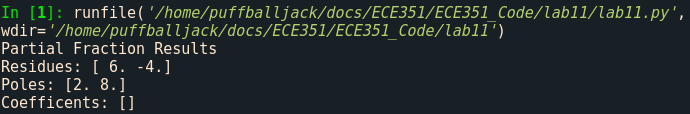
\includegraphics[width=\linewidth]{t3.png}
  \caption{Verification of PFE using \texttt{scipy.signal.residuez()}}
  \label{fig: t3}
\end{figure}
\begin{figure}[h!]
  \centering
  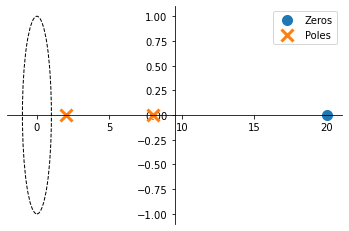
\includegraphics[width=\linewidth]{t4.png}
  \caption{H(z) Pole-Zero Plot using \texttt{zplane()}}
  \label{fig: t4}
\end{figure}
\begin{figure}[h!]
  \centering
  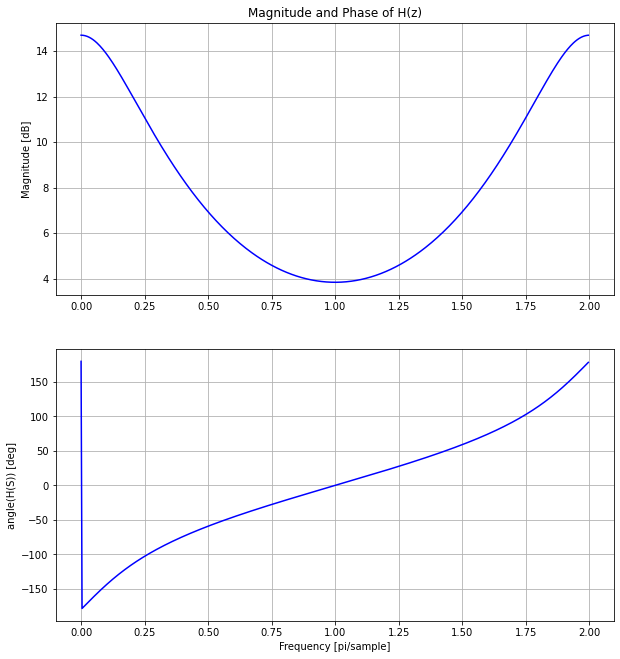
\includegraphics[width=\linewidth]{t5ns.png}
  \caption{Magnitude and Phase Response of H(z) [Base 10 Scale]}
  \label{fig: t5ns}
\end{figure}
\begin{figure}[h!]
  \centering
  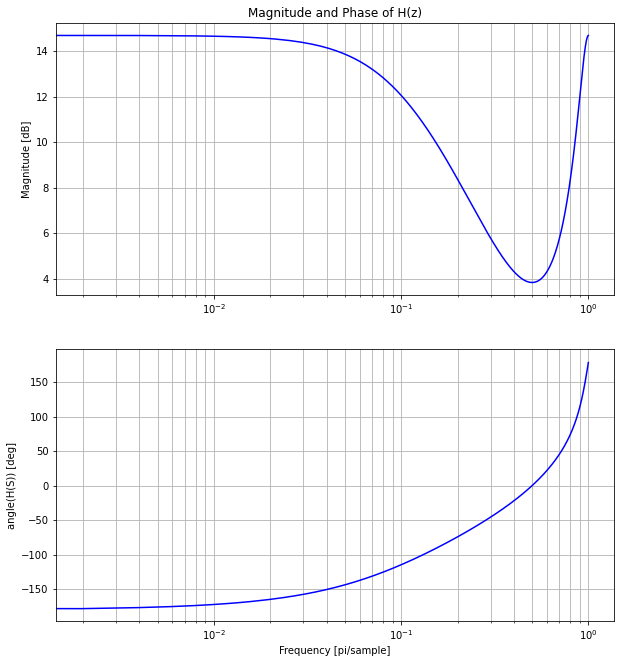
\includegraphics[width=\linewidth]{t5ls.png}
  \caption{Magnitude and Phase Response of H(z) [Logarithmic Scale]}
  \label{fig: t5ls}
\end{figure}


\section{Error Analysis}\label{section: ErAn}
No sources of error were seen throughout this lab. Verifying the PFE expansion performed by hand using the \texttt{scipy.signal.residuez()} function
actually removed, or at least reduced, a possible source of error.

\section{Questions}\label{section: Questions}
\begin{enumerate}
  \item Looking at the plot generated in Task 4, is H(z) stable? Explain why or why not.
  \begin{itemize}
    \item As seen in the plot generated in Task 4, Figure \ref{fig: t4}, all poles are in the right half plane. As is known, as z approaches those poles accumulation
    of energy will not end and causes instability. Thus, H(z) is unstable.
  \end{itemize}
  \item Leave any feedback on the clarity of lab tasks, expectations, and deliverables.
  \begin{itemize}
    \item This lab was very clear for all instructions, expectations and deliverables.
  \end{itemize}
\end{enumerate}
\section{Conclusion}
In conclusion, I feel this lab was very successful. After learning the z-transform content of this course, I almost feel it would have
been more useful to know this content first as many concepts seen throughout previous labs seem to rely heavily on these concepts.
All in all, I am very satisfied with what this lab has taught me and feel it was an excellent use of time.
\newpage
\thispagestyle{customblank}
\section{Attachments}\label{section: Attachments}
\centering\begin{enumerate}
  \item H(z) Hand Calculations
\end{enumerate}
\vspace*{\fill}

\includepdf[pages=2, offset=1in -1in]{./attachments/lab11.pdf}
% \includepdf[pages=3, offset=1in -1in]{./attachments/lab5.pdf}

% \begin{thebibliography}{111} 
% \thispagestyle{customplain}

% \end{thebibliography}
\end{document}
%This template was created by Roza Aceska.